\documentclass{beamer}

\usepackage{../packages/packages_mathalea}
\input{../competences/competences_latex.tex}
\usepackage{fontawesome}

\pgfplotsset{compat=1.18}

\begin{document}

\begin{frame}{\GetCompetence{Fonc18}}
On considère la fonction $f(x)=-2x^2-\dfrac{21}{5}x-\dfrac{9}{5}$.

\begin{enumerate}
	\item Déterminer la forme canonique de $f$. En déduire, les coordonnées du sommet du graphe de $f$.
	\item Déterminer les zéros de la fonction.

\medskip
\textbf {a.}  Le graphe de $f$ intersecte-t-il l'axe des abscisses ? Si oui, déterminer les coordonnées de ce(s) point(s) d'intersection.

\medskip
\textbf {b.}  En déduire le tableau des signes de la fonction $f$.
	\item Déterminer les coordonnées du point d'intersection de $f$ avec l'axe des ordonnées.
	\item Avec les résultats précédents, esquisser le graphe de $f$.
\end{enumerate}
\end{frame}

\begin{frame}
\begin{itemize}
	\item La forme canonique vaut $f(x)=-2\left(x+\dfrac{21}{20}\right)^2+\dfrac{81}{200}$. 

		Le sommet est $S\left(-\dfrac{21}{20};\dfrac{81}{200}\right)$.
	\item Le graphe intersecte l'axe des abscisses en 

		$R_1\left(-\dfrac{3}{5};0\right)$ et $R_2\left(-\dfrac{3}{2};0\right)$.
	\item On en déduit le tableau de signes suivant:
	\begin{center}
		\begin{tikzpicture}[scale=0.8]
			\tkzTabInit{$x$ / 1 , $f(x)$ / 1}{$-\infty$, $-\dfrac{3}{2}$, $-\dfrac{3}{5}$, $+\infty$}
			\tkzTabLine{, -, z, +, z, -, }
		\end{tikzpicture}
	\end{center}
	\item Le graphe intersecte l'axe des ordonnées en $(0;-9/5)$.
\end{itemize}
\end{frame}
\begin{frame}
	\begin{center}
	\begin{tikzpicture}[scale=1.4]
  \begin{axis}[
    axis lines=middle,
    xmin=-5, xmax=5,
    ymin=-5, ymax=5,
    xlabel={$x$}, ylabel={$y$},
    ticks=none,
    width=6cm, height=6cm,
    domain=-5:5,
  ]
  \addplot[only marks, red] coordinates {(-3/2,0) (-3/5,0) (0,-9/5) (-21/20,81/200)};
  \node[above right] at (axis cs:-10/2,0) {\tiny $R_1(-\dfrac{3}{2};0)$};
    \node[above right] at (axis cs:3/5,0) {\tiny$R_2(-\dfrac{3}{5};0)$};
    \node[above left] at (axis cs:3,-9/5) {\tiny$C(0;-\dfrac{9}{5})$};
    \node[above] at (axis cs:-38/20,2) {\tiny$S\left(\dfrac{-21}{20};\dfrac{81}{200}\right)$};

    \addplot[blue, thick, samples=100, domain=-5:5] {-2*x^2 - 4.2*x - 9/5};
  \end{axis}
\end{tikzpicture}
\end{center}

\end{frame}
\end{document}
